\setstretch{1.5}
\chapter{Sidewall Profile Control Strategy}

\tab In the previous chapter, it was shown that real-time multivariable feedback control can
be used to stabilize etch rate during reactive ion etching. While the stabilization of etch rate shows the utility of real-time feedback control, there are other important etch characteristics that also need to be controlled. As was described in Section 1.1.2, these include sidewall profile, selectivity, uniformity, and smface damage. In particular, control of sidewall profile has been an active area of research [1,61,66,93]. I have developed a strategy for sidewall profile control based on applying real-time feedback to the plasma generation process. In this chapter, a study of the feasibility of this strategy is presented.


\section{Sidewall Control Strategy}

\tab Sidewall profiles are difficult to characterize due to the small size (< 1 $\mu m$) of most features in integrated circuit devices. These profiles are often measured using scanning
electron microscopy (SEM). Unfortunately, SEM is inherently destructive (the wafer must
be cleaved through the structure of interest) and can therefore only be used on selective
samples. Recently, a non-destructive optical technique know as scatterometry has been explored to characterize reactive ion etch profiles [45,80,81]. 

\setstretch{1}
\begin{figure}[H]
	\centering
	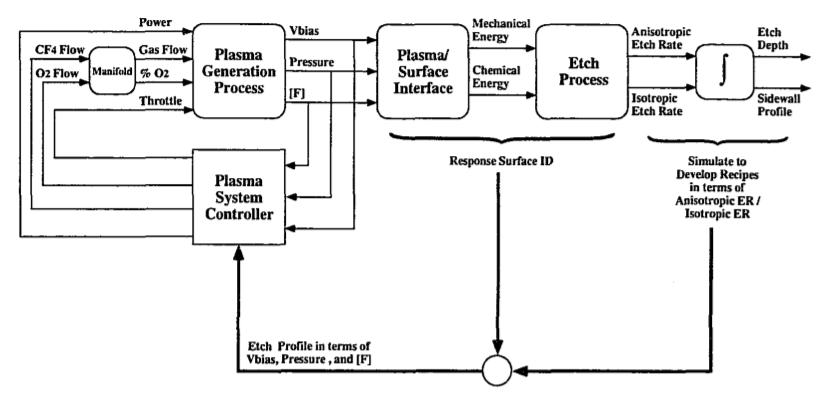
\includegraphics[scale = .5]{Figure 5.1}
	\bf\caption{  Sidewall Control Strategy.}
	\label{fig:5.1}
\end{figure}

\setstretch{1.5}
\noindent In scatterometry, laser light
is scattered off a periodic structure on the wafer surface. The sidewall profile can then
be estimated from the intensity of the scattered light at various diffraction angles. Scatterometry requires the measurement of diffracted light intensity over the entire 180 degrees above the wafer. Therefore, as there are a limited number of viewports on most chambers, scatterometry is not suited for \textit{in situ} measurements during the etch process. In addition, the analysis can be problematic when a mask layer is present over the profile. Therefore, scatterometry is not suited for real-time profile measurement during reactive ion etching, and an indirect strategy must be used to control sidewall profile.


The strategy for sidewall profile control that has been developed is based on a decomposition similar to that used in Section 3.1. This strategy can be broken down into two
parts: 1) determining the plasma characteristics necessary to achieve a desired sidewall
profile and 2) using a feedback controller to set these characteristics during an etch. The
mapping of sidewall profile to plasma properties is, in turn, divided into two parts. First, the etch rate components associated with the sidewall profile are found using a string model
simulation. Next, the plasma characteristics necessary to generate these etch rate components are determined using a response surface. Once the necessary plasma properties are
found, the etch can be performed using a feedback controller to regulate the plasma to these
conditions. In order to implement this strategy, a linear model of the plasma generation
process must first be developed. Prom this model, a real-time feedback controller can be
designed to hold plasma characteristics at desired values despite disturbances. Next, for
each of a variety of plasma conditions the resulting sidewall profile must be mapped into
etch rate components. Results from different operating points can then be used to construct
a response surface relating plasma characteristics to etch rate components. In the rest of
this chapter, the feasibility of this strategy is shown by relating the etch rate components
to a sidewall profile etched using real-time feedback control.

\section{Process Chemistry}
\tab In using plasma characteristics to control sidewall profile, it is likely that all three
properties ($\text{V}_{bias}$, pressure, and fluorine concentration) play an important role. As was seen in Section 3.2.2, in a pure $\text{CF}_{4}$ chemistry only two of these characteristics could be independently controlled. In order to achieve control over a third characteristic, $\text{O}_{2}$ was added to the feed gas. Oxygen causes the following reactions to occur in the plasma [85,90,91]

\setstretch{1}
\begin{align}
	\text{CF}_{3} + \text{O} &\rightarrow \text{COF}_{2} + \text{F}, \\
	\text{CF}_{2} + \text{O} &\rightarrow \text{COF} + \text{F}, \\
	\text{COF} + \text{O} &\rightarrow \text{CO}_{2} + \text{F}, 
\end{align}

\noindent and

\begin{align}
	\text{CF}_{2} + O \rightarrow \text{CO} +\text{F}
\end{align}

\setstretch{1.5}
\noindent These reactions lead to a higher fluorine concentration by liberating more fluorine radicals and by blocking the recombination reaction

\setstretch{1}
\begin{align}
	\text{CF}_{x} + F \rightarrow \text{CF}_{x+1}
\end{align}

\setstretch{1.5}
\noindent where $x = {0 ,...3 }$. Oxygen has a small effect on total dissociation and the electrical properties of the discharge; thus its addition does not greatly effect $\text{V}_{bias}$ and pressure. The use of \%$\text{O}_{2}$, in addition to throttle position and applied power, should allow independent control of all three plasma characteristics. This was verified by using the dc gain matrix for the plasma generation process

\setstretch{1}
\begin{align}
	\renewcommand\arraystretch{1.5} \begin{bmatrix}
		V_{bias} \\ \text{Pressure} \\ \text{Fluorine}
	\end{bmatrix} = 
	\renewcommand\arraystretch{1.5} \begin{bmatrix}
		0.3713 & 0.0088 & 0.8232 \\ -1.2194 & 0.0168 & 0.0084 \\ -0.6279 & 0.5932 & 1.0835
	\end{bmatrix}
	\renewcommand\arraystretch{1.5} \begin{bmatrix}
		\text{Throttle} \\ \text{\%O}_{2} \\ \text{Power}
	\end{bmatrix}
\end{align}

\noindent The singular values for this matrix were

\begin{align}
	\renewcommand\arraystretch{1.5} \begin{bmatrix}
		1.6016 & 1.2560 & 0.2835
	\end{bmatrix},
\end{align}

\noindent yielding condition number of

\begin{align}
	\kappa = 5.7.
\end{align}

\setstretch{1.5}
\noindent Thus, the dc gain matrix was invertible and independent control of the three plasma characteristics was possible.

In general, sidewall passivation is often used to control etch profiles. As was discussed
in Section 1.2.3, in a $\text{CF}_{4}$ chemistry the passivation occurs when polymers form on the poly silicon in areas where ion bombardment is not present. While the addition of hydrogen into the plasma chemistry potentially allows for the control of polymerization, there is a significant amount of preliminary research that needs to be performed before this procedure may be used in a real-time control strategy. This is beyond the scope of this dissertation. To focus our research, we decided to simplify the plasma/surface interactions by not exploiting sidewall passivation. The addition of oxygen to the plasma chemistry not only provides an extra degree of plasma control, but also reduces polymerization from the plasma [23].

In order to show that a variety of sidewall profiles could be achieved using the $\text{CF}_{4}\ \text{O}_{2}$
chemistry, a number of etches were performed using the standard industrial practice of
setting pressure, flow rates, and applied power. Figure 5.2 shows an isotropic sidewall
profile resulting from an etch performed at 20 mTorr, \%5 $\text{O}_{2}$, 30 sccm total fiow, and
1000 W applied power. Likewise, Figure 5.3 shows a near vertical profile resulting from an
etch performed at 10 mTorr, \%1 $\text{O}_{2}$, 30 sccm total flow, and 1200 W applied power. These etches show that the $\text{CF}_{4}$/$\text{O}_{2}$ chemistry is capable of etching a wide variety of sidewall profiles.

\section{Plasma Generation Process Model}
\tab As in the previous chapter, the process of designing a controller begins by developing a
model of the plasma generation process for the $\text{CF}_{4}/\text{O}_{2}$ chemistry. As before, the first step in developing this model was the selection of an operating point around which the model would be identified. The operating conditions for throttle position and applied power were chosen to be the same as in the pure $\text{CF}_{4}$ case. It has been 


\setstretch{1}
\begin{figure}[H]
	\centering
	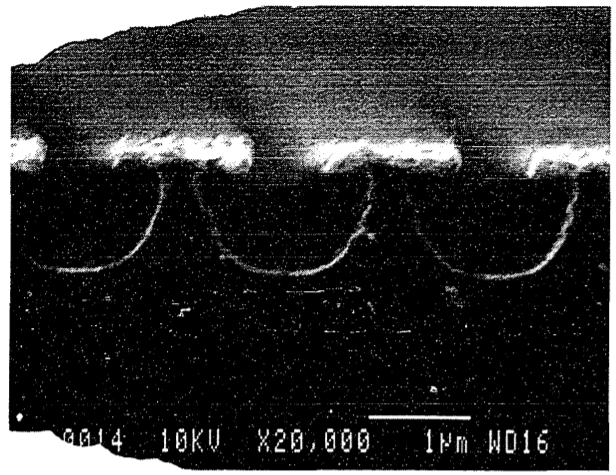
\includegraphics[scale = .5]{Figure 5.2}
	\bf\caption{  Sidewall profile resulting from an etch with settings of 20 mTorr,
		5 \%$\text{O}_{2}$, 30 sccm total flow, and 1000 W power.}
	\label{fig:5.2}
\end{figure}

\begin{figure}[H]
	\centering
	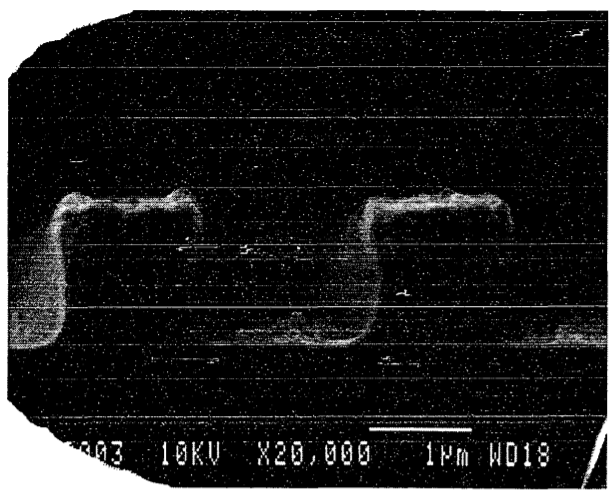
\includegraphics[scale = .5]{Figure 5.3}
	\bf\caption{  Sidewall profile resulting from an etch with settings of 10 mTorr,
		\%$\text{0}_{2}$, 30 sccm total flow, and 1200 W power.}
	\label{fig:5.3}
\end{figure}

\begin{table}[H]
	\centering
	\renewcommand\arraystretch{1.5}
	\begin{tabular}{|c|c|}
		\hline
		Throttle Position & 12.5 \%Open \\
		\hline
		\% $\text{O}_{2}$ & 5 \% \\
		\hline
		Applied Power & 1000 W \\
		\hline
		Total Flow Rate & 30 sccm \\
		\hline
	\end{tabular}
	\bf\caption{ Operating point for $\text{CF}_{4}$/$\text{O}_{2}$ plasma.}
	\label{table:5.1}
\end{table}

\setstretch{1.5}
\noindent shown that while fluorine concentration continues to increase up to the addition of ~ 25\% $\text{O}_{2}$, the etch rate decreases after the addition of ~ 12\% $\text{O}_{2}$ [79]. Hence, the operating point was selected at 5\% $\text{O}_{2}$ with a total gas flow (flow of $\text{CF}_{4}$ + Ar + $\text{O}_{2}$) of 30 sccm. The operating point is given in Table 5.1.

Using the same techniques outlined in Section 3.2.2 the following model was identified
for the $\text{CF}_{4}/\text{O}_{2}$ plasma generation process

\setstretch{1}
\begin{align}
	\renewcommand\arraystretch{2}\begin{bmatrix}
		V_{bias} \\ \text{Pressure} \\ \text{Fluorine}
	\end{bmatrix} = 
	\renewcommand\arraystretch{2}\begin{bmatrix}
		\frac{1.65e^{-0.42s}}{s+0.16} & \frac{0.25e^{-0.77s}}{s+0.41} & \frac{12.23(s+0.27)}{(s+0.19)(s+62.42)} \\
		\frac{-0.97e^{-0.42s}}{(s+0.18)(s+3.00)} & \frac{0.024e^{-0.77s}}{s+0.40} & \frac{-0.011(s-0.006)}{(s+0.19)(s+2.33)} \\
		\frac{4.85(s-0.73)e^{-0.42s}}{(s+0.11)(s+39.76)} & \frac{0.33e^{-0.77s}}{s+0.17} & \frac{0.49(s+0.067)}{(s+0.095)(s+19.69)}
	\end{bmatrix}
	\renewcommand\arraystretch{2}\begin{bmatrix}
		\text{Throttle} \\ \text{\% O}_{2} \\ \text{Power}
	\end{bmatrix}
\end{align}

\setstretch{1.5}
\noindent As shown in Figure 5.4, in this case the time delay from the throttle valve was found to be
0.42 seconds, as opposed to the 0.62 seconds in Chapter 3. It is unlikely that the addition
of $\text{O}_{2}$ to the plasma chemistry would have such an effect on the delay in response to throttle
changes. Instead, this difference might be accounted for by the fact that the models were
developed over a year and a half apart.

\section{Plasma Controller}

\tab A plasma generation process controller for the $\text{CF}_{4}$/$\text{O}_{2}$ chemistry was designed to meet the same performance objective and design constraints outlined in Section 4.1. The state

\setstretch{1}
\begin{figure}[H]
	\centering
	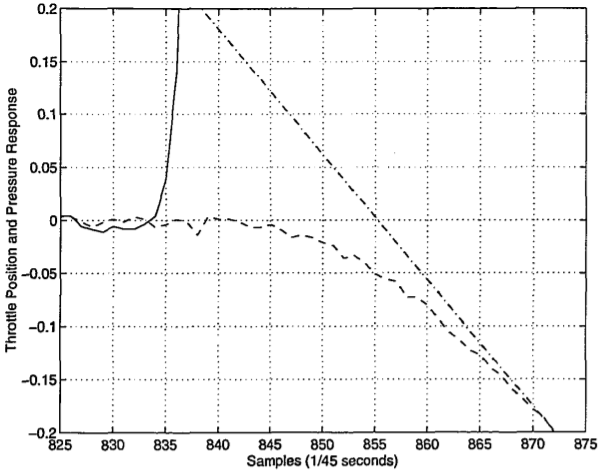
\includegraphics[scale = .5]{Figure 5.4}
	\bf\caption{  Delay in response of pressure to change in throttle position.}
	\label{fig:5.4}
\end{figure}

\noindent feedback and observer gains were found using the same design methodology with weights

\begin{align}
	\alpha &= 3, \\
	Q_{q} &= \renewcommand\arraystretch{1.5} \begin{bmatrix}
		1.3 & 0 & 0 \\ 0 & 0.3 & 0 \\ 0 & 0 & 0.5
	\end{bmatrix} \\
	R &= \renewcommand\arraystretch{1.5} \begin{bmatrix}
		1.5 & 0 & 0 \\ 0 & 1.5 & 0 \\ 0 & 0 & 0.5
	\end{bmatrix}
\end{align}

\noindent and

\begin{align}
	\rho = 1.
\end{align}

\setstretch{1.5}
As can be seen in Figures 5.5 through 5.10 the controller achieves its performance objectives.
The controller had 19 states, but was reduced to 8 states using the model reduction method
outlined in Section 4.1.1. Inspection of the Bode plots for the full and reduced order controllers (shown in Figures 5.11 through 5.13), shows that the controllers have similar responses in their crossover regions.

\subsection{Anti-Windup Design}

\tab As was mentioned in Section 4.2.1, a large disturbance due to outgassing from the
chamber walls was present during every etch performed on our AME-8300. This disturbance
primarily effects the fluorine concentration. As can be seen from the dc gain matrix in
Equation 5.6, the controller will respond to this disturbance by reducing the \%$\text{O}_{2}$ in the
feed gas. Because the gain from this actuator to fluorine concentration was not very large,
there was the potential that \%$\text{O}_{2}$ would saturate during the initial portion of an etch.
Therefore, anti-windup logic was added to the controller to minimize the effect of this
saturation.

The controller designed above had the form

\setstretch{1}
\begin{align}
	\dot{x} &= A_{c}x + B_{c}y + G_{c}r \\
	u &= C_{c}x + D_{c}y.
\end{align}

Rather than let the actuators saturate, each input was software limited

\begin{align}
	\hat{u} = \begin{cases}
		u_{lower} \quad \text{if} \ u \leq u_{lower}, \\
		u \quad \text{if} \ u_{lower} < u < u_{upper}, \\
		u_{upper} \quad \text{if} \ u \geq u_{upper},
	\end{cases}
\end{align}

\setstretch{1.5}
\noindent as shown in Figure 5.14. These limits are shown in Table 5.2. The compensator was then
modified by multiplying Equation 5.15 by the anti-windup gain $\text{K}_{u}$ and subtracting it from
Equation 5.14 [6]. This yields


\setstretch{1}
\begin{align}
	\dot{x} = (A_{c}-K_{u}C_{c})x + (B_{c}-K_{u}D_{c})y + K_{u}\hat{u} + G_{c}r,
\end{align}

\begin{figure}[H]
	\centering
	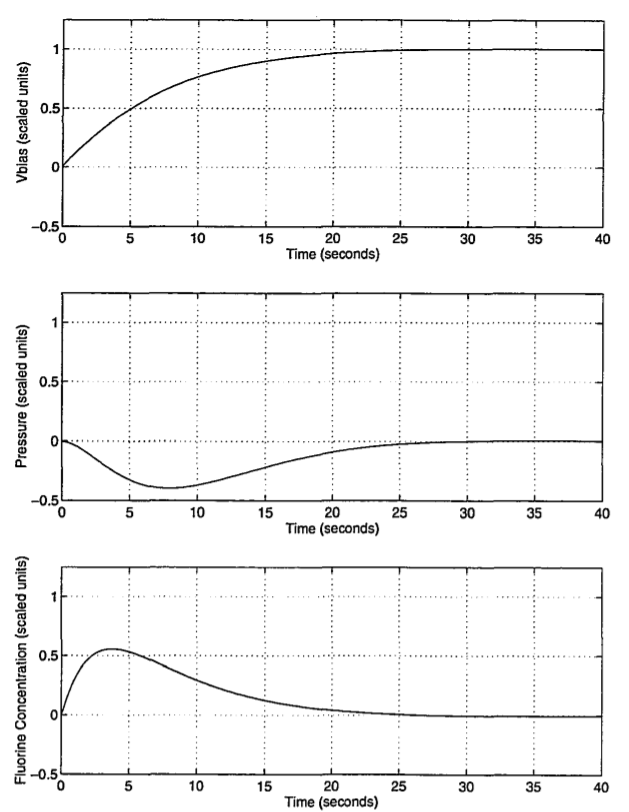
\includegraphics[scale = .5]{Figure 5.5}
	\bf\caption{  Simulated response of closed loop system to step in $\text{V}_{bias}$.}
	\label{fig:5.5}
\end{figure}

\begin{figure}[H]
	\centering
	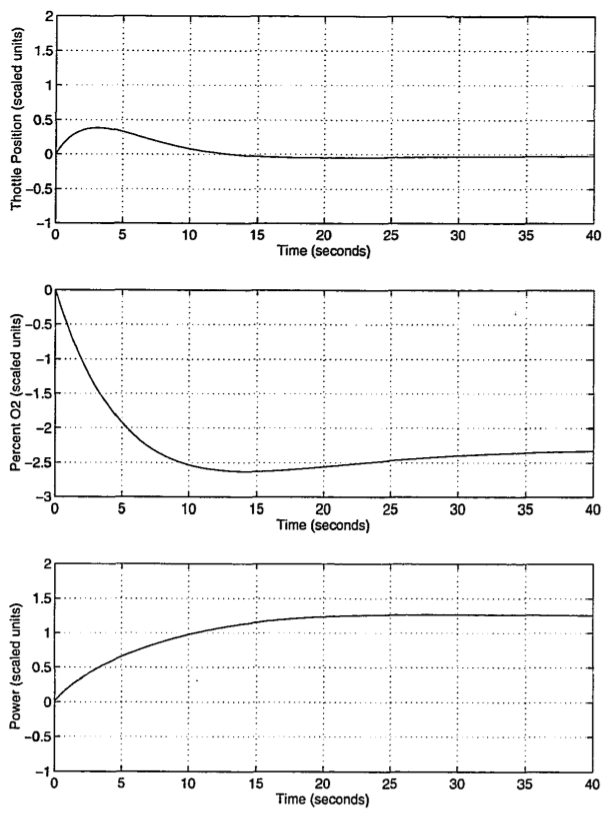
\includegraphics[scale = .75]{Figure 5.6}
	\bf\caption{  Simulated response of actuators to step in $\text{V}_{bias}$.}
	\label{fig:5.6}
\end{figure}

\begin{figure}[H]
	\centering
	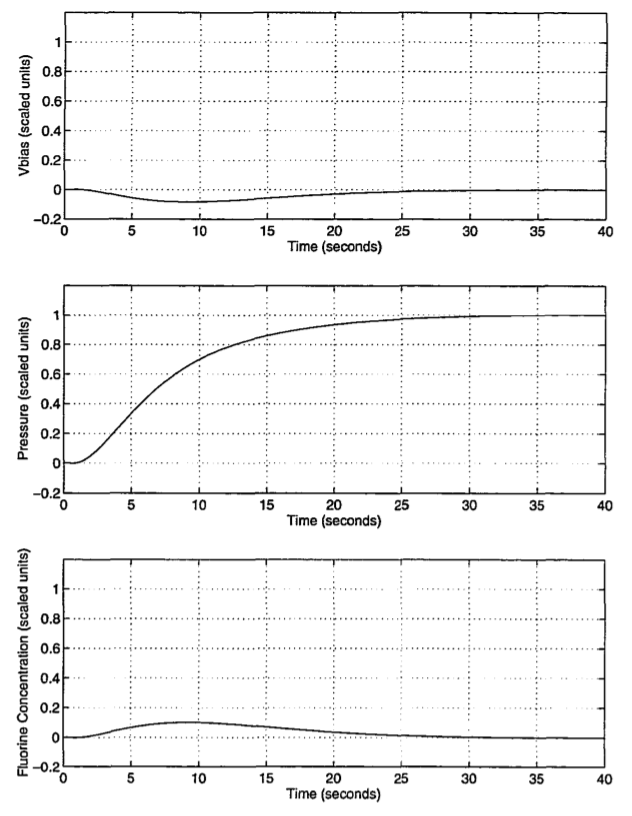
\includegraphics[scale = .75]{Figure 5.7}
	\bf\caption{  Simulated response of closed loop system to step in pressure.}
	\label{fig:5.7}
\end{figure}

\begin{figure}[H]
	\centering
	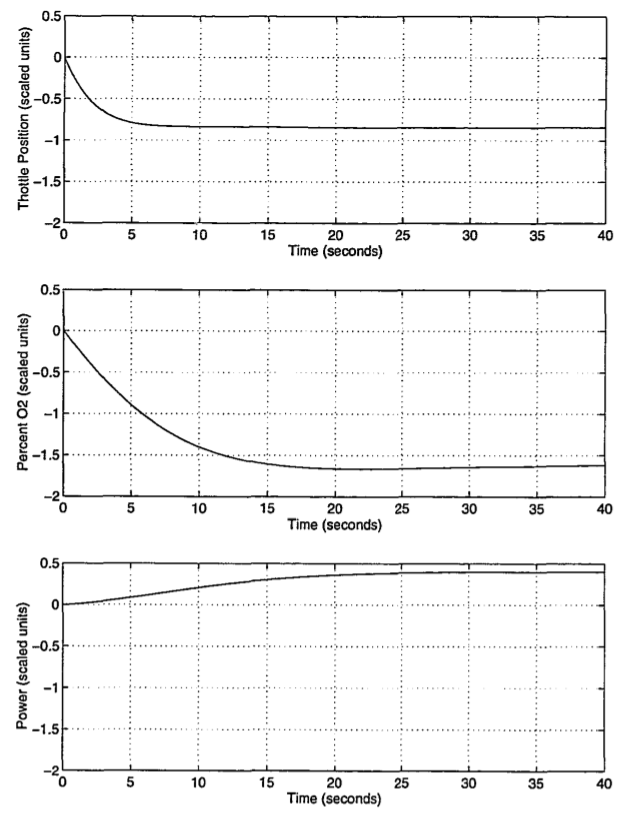
\includegraphics[scale = .75]{Figure 5.8}
	\bf\caption{  Simulated response o f actuators to step in pressure.}
	\label{fig:5.8}
\end{figure}

\begin{figure}[H]
	\centering
	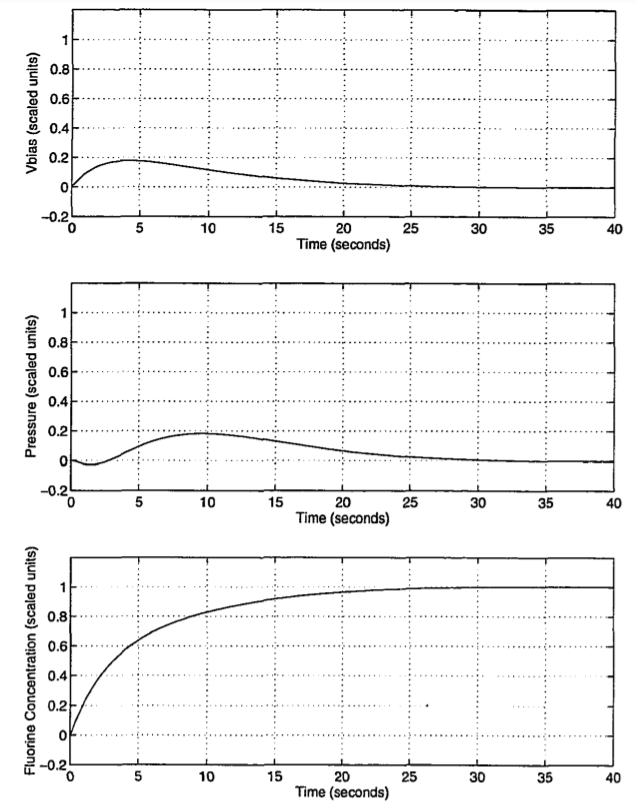
\includegraphics[scale = .75]{Figure 5.9}
	\bf\caption{  Simulated response of closed loop system to step in fluorine	concentration.}
	\label{fig:5.9}
\end{figure}

\begin{figure}[H]
	\centering
	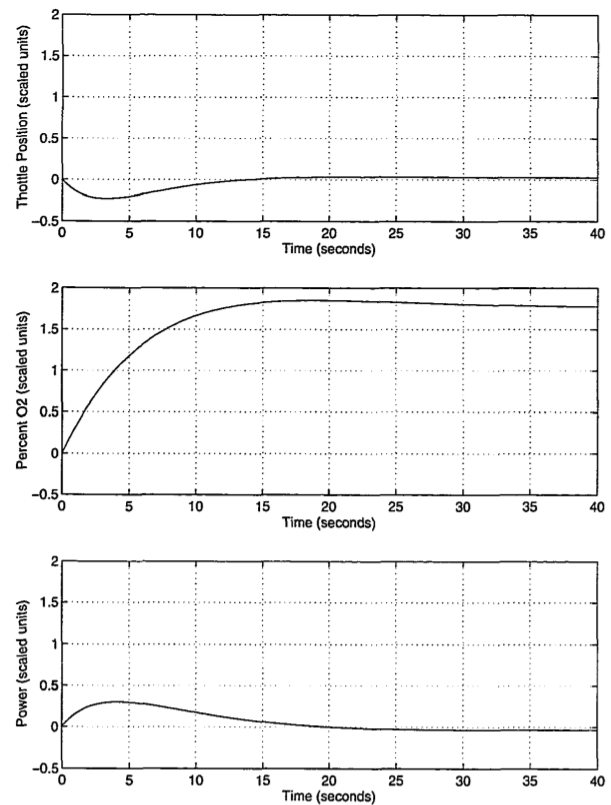
\includegraphics[scale = .75]{Figure 5.10}
	\bf\caption{  Simulated response of actuators to step in fluorine concentration.}
	\label{fig:5.10}
\end{figure}

\begin{figure}[H]
	\centering
	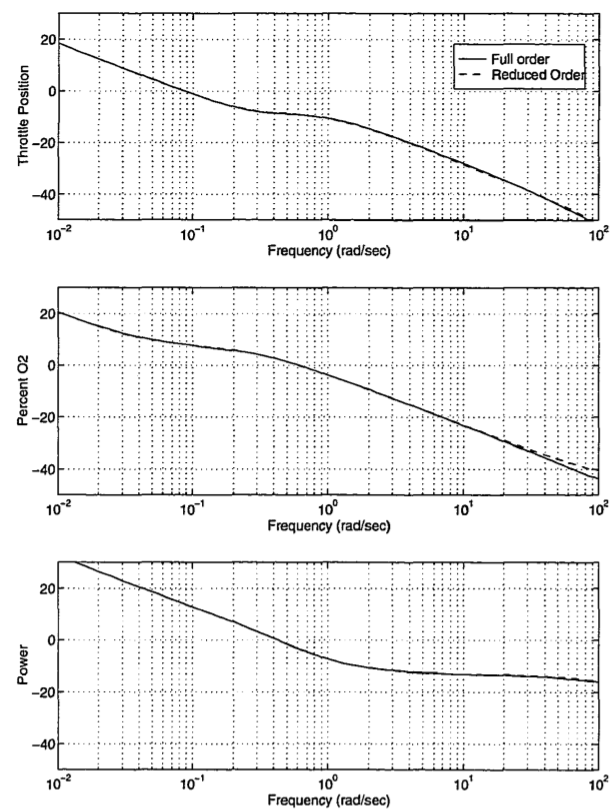
\includegraphics[scale = .75]{Figure 5.11}
	\bf\caption{  Bode plots of controller from $\text{V}_{bias}$ to equipment inputs.}
	\label{fig:5.11}
\end{figure}

\begin{figure}[H]
	\centering
	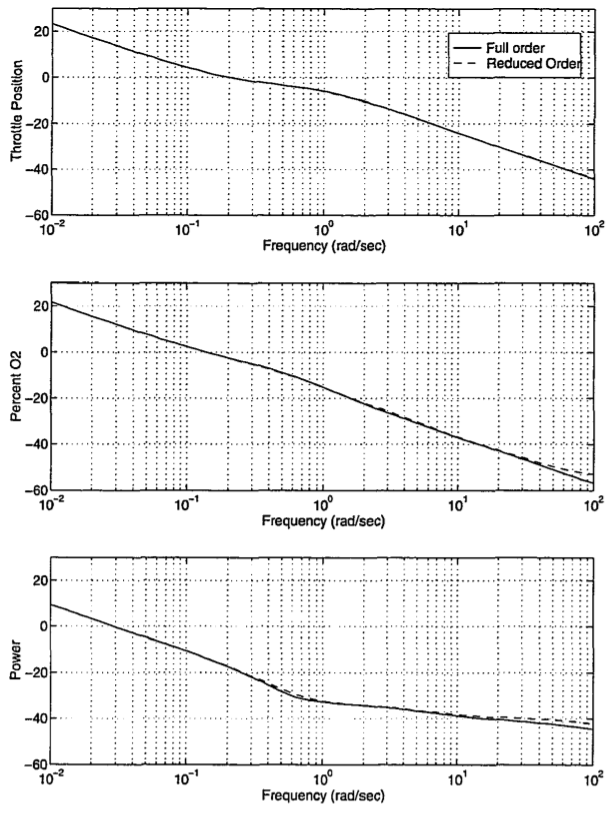
\includegraphics[scale = .75]{Figure 5.12}
	\bf\caption{  Bode plots of controller from pressure to equipment inputs.}
	\label{fig:5.12}
\end{figure}

\begin{figure}[H]
	\centering
	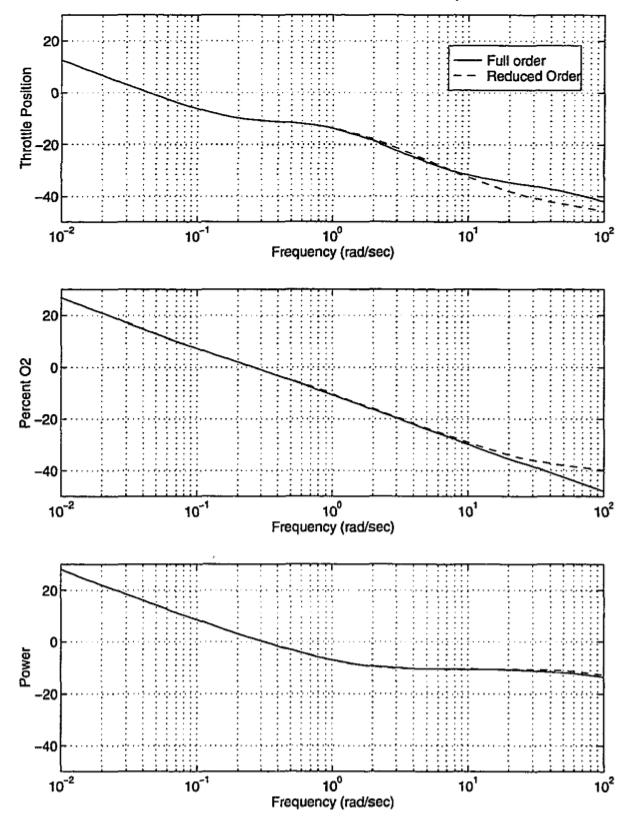
\includegraphics[scale = .75]{Figure 5.13}
	\bf\caption{  Bode plots of controller from fluorine concentration to equipment inputs.}
	\label{fig:5.13}
\end{figure}

\begin{figure}[H]
	\centering
	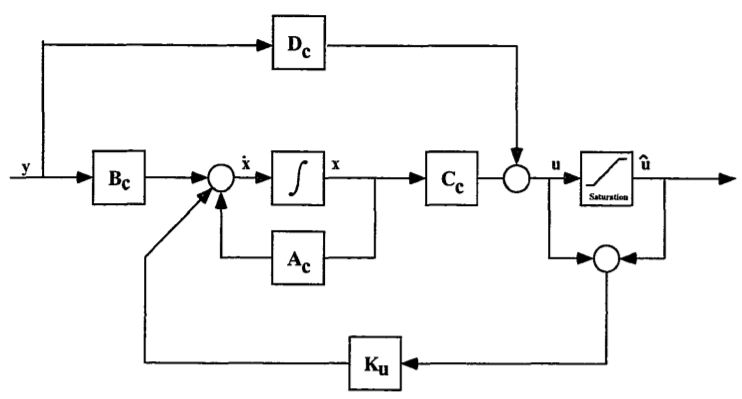
\includegraphics[scale = .5]{Figure 5.14}
	\bf\caption{  Controller with anti-windup logic.}
	\label{fig:5.14}
\end{figure}

\setstretch{1.5}
\noindent When the actuators are not saturated ($\hat{u} = u$), Equation 5.17 reduces to Equation 5.14 and
the anti-windup logic has no affect on the performance of the controller. When the actuators
saturate, the anti-windup logic helps to keep the states of the controller from continuing to
grow. The gain $K_{u}$ was found by solving the linear quadratic regulator problem for ($A'_{c}, C'_{c}$)
using weighting matrices

\setstretch{1}
\begin{align}
	Q_{u} = 2 \times I_{8}
\end{align}

\noindent and

\begin{align}
	R_{u} = I_{3}
\end{align}

\noindent where $I_{n}$ is the identity matrix of the dimension $n$. This yielded and input feedback gain of

\begin{align}
	K_{u} = \renewcommand\arraystretch{1.5} \begin{bmatrix}
		0.107 & 0.049 & 0.161 & -0.094 & -0.128 & -0.457 & 1.262 & 0.445 \\ 0.031 & -0.016 & 0.082 & -0.072 & 0.048 & 0.918 & 0.638 & -0.867 \\ -0.181 & 0.011 & 0.267 & 0.145 & 0.051 & -0.974 & 0.009 & -1.025
	\end{bmatrix}.
\end{align}

\setstretch{1.5}
\noindent The ability of the controller, with and without anti-windup logic, to reject an exponentially
decaying disturbance to fluorine concentration was simulated. As can be seen from Figure 5.15, the controller with anti-windup logic comes off saturation more quickly than the one without the added logic.

\setstretch{1}

\begin{table}[H]
	\centering
	\renewcommand\arraystretch{1.5}
	\begin{tabular}{|c|c|c|}
		\hline
		Actuator & Lower Limit & Upper Limit\\
		\hline
		Throttle Position & 1 \%Open & 50 \%Open \\
		\hline
		\%$\text{O}_{2}$ & 1\% & 12.5\% \\
		\hline
		Applied Power & 300 & 1500 W \\
		\hline 
	\end{tabular}
	\bf\caption{Software saturation limits.}
	\label{table:5.2}
\end{table}

\setstretch{1.5}
\subsection{Implementation}
\tab This controller was implemented using the LabVIEW data acquisition and control system. The actuator commands from the controller were software limited by the LabVIEW code and fed back to the controller as shown in Figure 5.16.


The \%$\text{O}_{2}$ command from the controller must be converted to $\text{CF}_{4}/\text{Ar}$ and $\text{O}_{2}$ commands for the mass flow controllers. The total flow was held constant at 30 sccm and the percentage of oxygen was taken with respect only to the $\text{CF}_{4}$ flow. Lab VIEW calculated the two flow commands as

\setstretch{1}
\begin{align}
	\text{CF}_{4}/\text{Ar} = \frac{\text{Total Flow}}{1+\text{\% O}_{2}(1-\alpha)}
\end{align}

\noindent and

\begin{align}
	\text{O}_{2} = \text{Total Flow} - \text{CF}_{4}/\text{Ar}
\end{align}

\noindent where $\alpha$ is the percentage of argon in the premixed $\text{CF}_{4}/\text{Ar}$ bottle.

\begin{figure}[H]
	\centering
	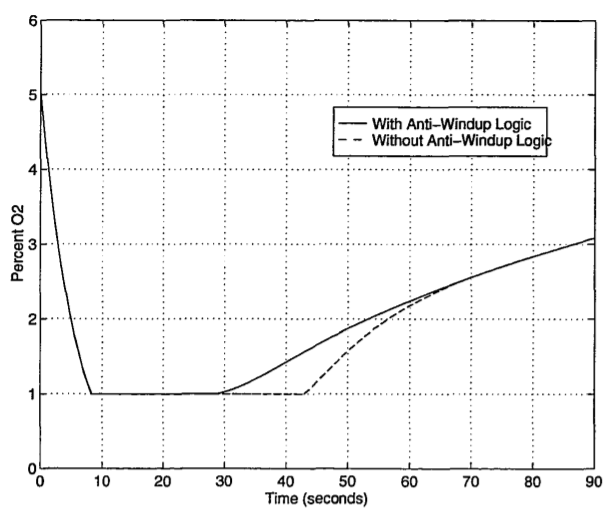
\includegraphics[scale = .75]{Figure 5.15}
	\bf\caption{  Simulated response of \% $\text{O}_{2}$ to fluorine disturbance for controller with and without anti-windup logic.}
	\label{fig:5.15}
\end{figure}

\begin{figure}
	\centering
	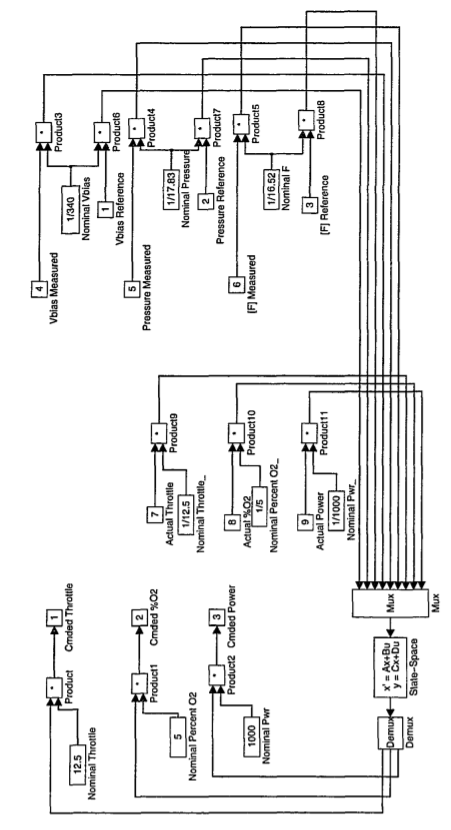
\includegraphics[scale = 0.75]{Figure 5.16}
	\bf\caption{Controller structure with anti-windup.}
	\label{fig:5.16}
\end{figure}

\setstretch{1.5}
\section{Etch Study}
\tab In the overall control strategy, a response surface will be used to map plasma characteristics to etch rate components. An etch study will be performed to obtain the sidewall profiles resulting from etches at a variety of plasma conditions. These profiles will then bevanalyzed to yield the associated etch rate components; thus allowing the construction of a model relating plasma properties to isotropic and anisotropic etch rates. In this section, the feasibility of this method is shown by performing these steps for a single set of operating conditions.

\subsection{Wafer Preparation}
\tab In this etch study, the real-time feedback controller was used to control the etcher at
constant plasma characteristics during the etching of a masked polysilicon/$\text{SiO}_{2}$/Si wafer.
The selectivity of polysilicon to photoresist in a $\text{CF}_{4}/\text{O}_{2}$ plasma is very poor. Therefore, the features in a photoresist mask would change significantly during the etch. To focus
this research, a metal mask, which will not etch in a $\text{CF}_{4}$ chemistry, was used. This mask
allowed us to concentrate on modeling the effect that plasma properties have on etch rate
components without having to account for the efiects of mask erosion. A lift-off process
[102] (shown in Figure 5.17) was used to define the metal mask, which contains 1 $\mu m$, 2
$\mu m$, and 5 $\mu m$ linewidths with various spacings.


Nickel masks were initially used during this research. However, nickel masks have been
shown to enhance etch rate, and thus affect sidewall profile, in a $\text{CF}_{4}/\text{O}_{2}$ chemistry [31]. It is suspected that this is due to nickel acting as a catalyst for the dissociation of $\text{CF}_{x}$. As an alternative, etches were performed using aluminum and chromium for the mask layer, since these two metals have less of a catalytic effect. With both of these etches, a large amount of polymer was observed under the masks (see Figure 5.18). This amount of polymerization
is not typical for a $\text{CF}_{4}/\text{O}_{2}$ plasma and the exact cause has not been determined. To limit, the scope of this feasibility study, attempts were made to minimize polymer deposition, so we continued to use nickel masks.

The first step in the lift-off process is to make a photoresist mask layer with the inverse of the desired pattern. This was done using a Karl-Suss MA-6 contact aligner with an exposure wavelength of 350 nm. Initially, a clear field mask with the inverse pattern and Shipley Microposit S1822 photoresist were used. This led to the following problem. In order to define the smaller linewidths it was required that the aligner be in the hard-contact mode; however, in this mode, the wafers would adhere to the clear field 

\setstretch{1}
\begin{figure}[H]
	\centering	
	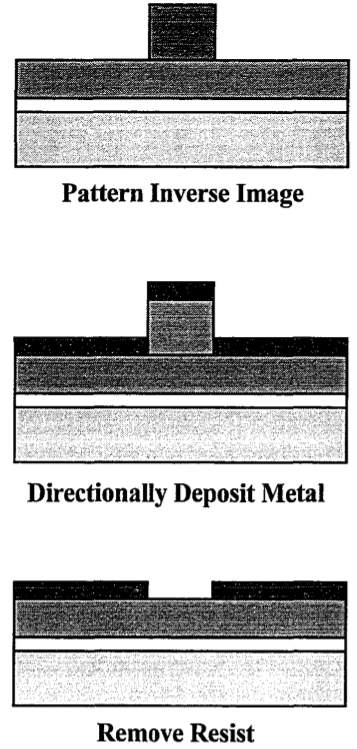
\includegraphics[scale = 0.75]{Figure 5.17}
	\bf\caption{ The lift-off process.}
	\label{fig:5.17}
\end{figure}

\begin{figure}[H]
	\centering	
	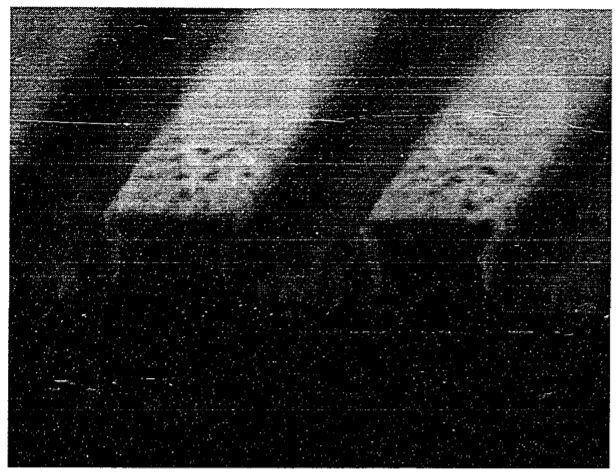
\includegraphics[scale = 0.5]{Figure 5.18}
	\bf\caption{ Polymer formation under a chromium mask.}
	\label{fig:5.18}
\end{figure}

\setstretch{1.5}
\noindent mask after exposure. It is thought that some of the photoresist was vaporized during exposure and that after cooling it “glued” the wafer to the mask.

A dark field mask and Hoechst AZ 5214 image reversing photoresist [99] was used to overcome the adhesion problem. Before patterning, the wafers were put through a dehydration bake at 110 °C to remove any moisture from their surfaces. Then the 5214 photoresist was spin-coated onto the surface at 4000 rpm for 30 seconds. After a soft bake for 30 minutes at 90 °C, this resulted in a 1.4 $\mu m$ thick resist layer. The wafers were then exposed for 10.4 seconds with a light intensity of 5 mA. A 30 minute bake at 100 °C was used to cross link polymers in the exposed portion of the photoresist. Next, the wafers were flood exposed, with no mask, for 30 seconds. Finally, the wafers were developed for 1.0 minute with MF 312 developer.

The metal mask was defined by evaporating nickel onto the wafer surface. Prior to evaporation, the wafers were plasma ashed (at 80 W and 250 mTorr) to remove any photoresist residue. Next, 1000$\dot{\text{A}}$ of nickel was deposited onto the wafer using a Denton SJ-20 e-beam evaporator. An SEM image of the wafer after nickel deposition is shown in Figure 5.19. Finally, the photoresist, and the nickel above it, was removed using heated XX 1112A developer and ultrasonic agitation.

\subsection{Controlled Etch}

\tab As an initial starting point for the etch study, the plasma conditions associated with
the nominal operating point for the system identification were used. These turned out to
be a bias voltage of 361 V, a chamber pressure of 18.25 mTorr, and a fluorine concentration
of 9.59 (arbitrary units). As can be seen in Figure 5.20, the controller compensates for the
wall disturbance and drives all three plasma characteristics to their desired setpoints. The
corresponding actuator commands are shown in Figure 5.21. After the etch, the wafer was
cleaved and imaged using a Joel MSJ-6 scanning electron microscope.

\setstretch{1}
\begin{figure}[H]
	\centering	
	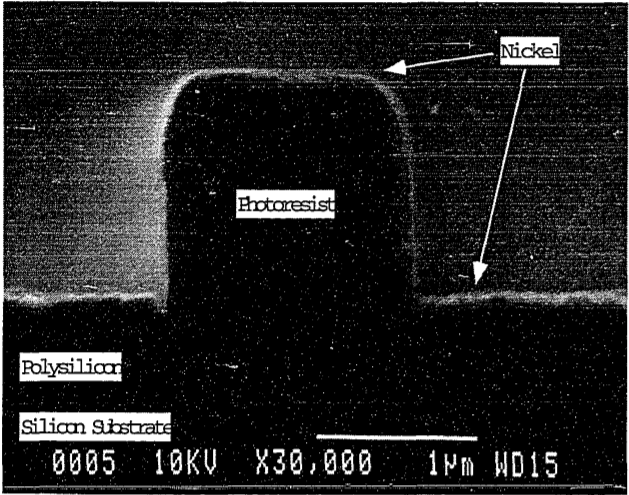
\includegraphics[scale = 0.6]{Figure 5.19}
	\bf\caption{ Wafer after nickel deposition.}
	\label{fig:5.19}
\end{figure}

\setstretch{1.5}
\subsection{String Model Simulation}
\tab The final step is to extract the isotropic and anisotropic etch rate components from the
SEM image. This is done by using a string model [59] to obtain a simulated sidewall profile
from specified etch rate components. In the string model, the exposed polysilicon surface
is represented by a series of nodes connected by straight line segments. The progression
of each node is determined by its local etch rate. This etch rate is the vector sum of an
isotropic component along the angle bisector of the two adjacent segments and an anisotropic
component in regions not masked by the nickel (see Figure 5.23). As the separation between
points changes during the etch simulation, nodes are added and subtracted from the string
to maintain sufficient resolution and relieve computational load. This model has been
implemented in C and uses etch rate components and etch time to produce a profile. The
source code is list in Appendix B.

\setstretch{1}
\begin{figure}[H]
	\centering	
	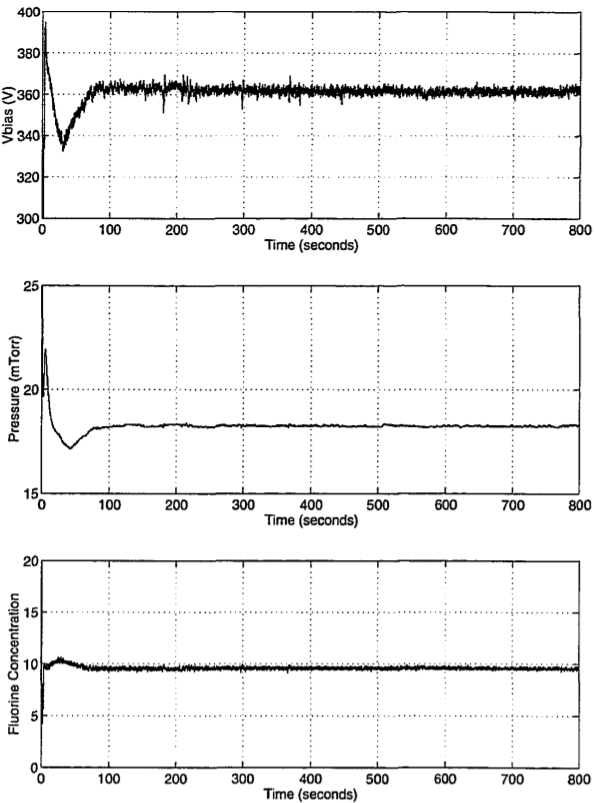
\includegraphics[scale = 0.75]{Figure 5.20}
	\bf\caption{ Plasma characteristics during feedback control of the plasma generation process.}
	\label{fig:5.20}
\end{figure}

\begin{figure}[H]
	\centering	
	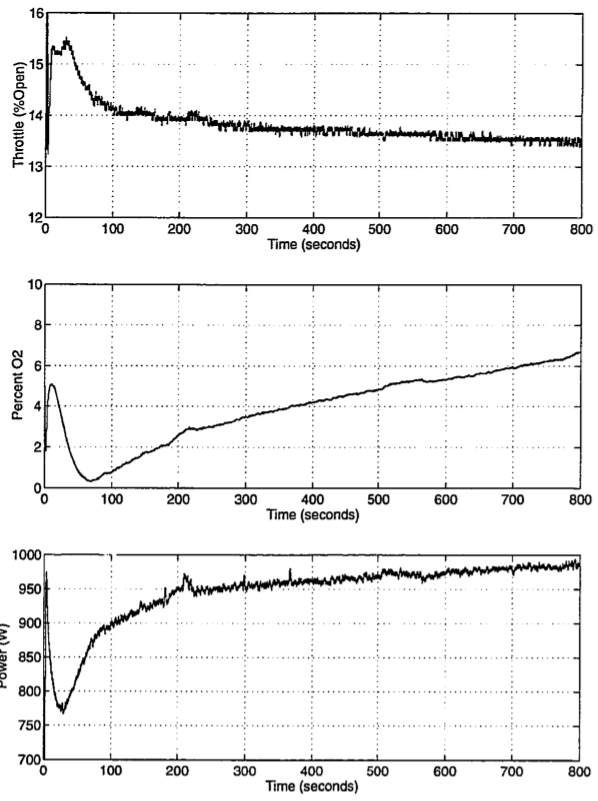
\includegraphics[scale = 0.75]{Figure 5.21}
	\bf\caption{ Corresponding actuator responses during feedback control.}
	\label{fig:5.21}
\end{figure}

\begin{figure}[H]
	\centering	
	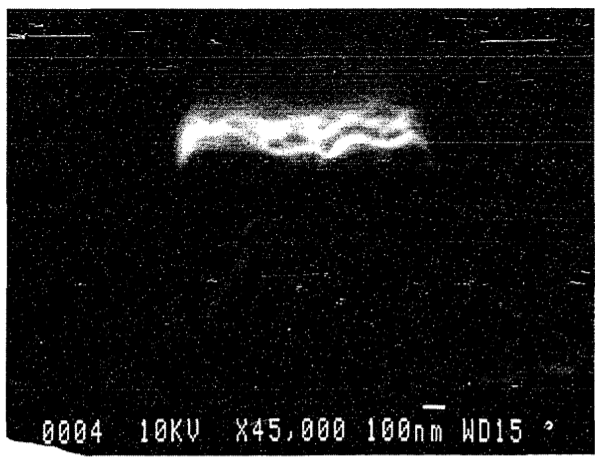
\includegraphics[scale = 0.6]{Figure 5.22}
	\bf\caption{ SEM image of resulting sidewall profile.}
	\label{fig:5.22}
\end{figure}

\begin{figure}[H]
	\centering	
	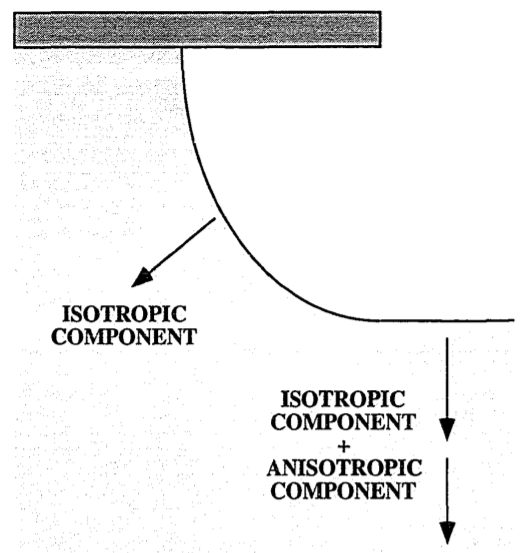
\includegraphics[scale = 0.6]{Figure 5.23}
	\bf\caption{ Isotropic and anisotropic etch rate components.}
	\label{fig:5.23}
\end{figure}

\setstretch{1.5}
\subsection{Determining Etch Rate from the SEM Image}
\tab The SEM image was captured on Polaroid 553 film and then scanned into a digital
format. Edges were extracted from this image using the Matlab Image Processing Toolbox
[103] to identify the regions of greatest intensity gradient. Then, using the m-files presented in Appendix A.2, the sidewall profile is extracted.

The string simulation is iterated to produce a good fit with the sidewall profile extracted
from the SEM image. As can be seen in Figure 5.24, the simulation does an excellent job
of capturing slope and shape of the sidewall profile. There is some mismatch between the
two in the corners, likely due to the simulation not accounting for local diffusion effects of
the reactive species. For this operating point, the etch rate components were found to be
6.0 $\dot{\text{A}}$/s isotropic and 6.5 $\dot{\text{A}}$/s anisotropic.

\section{Implementations of the Sidewall Profile Control~Strategy}
\tab This feasibility study has extended the RIE control work presented in Chapter 4 in
two directions. First, it has been shown that, by using \%$\text{O}_{2}$ as an actuator, it is possible to have independent control over the three plasma characteristics: $\text{V}_{bias}$, pressure, and fluorine concentration. Second, it has been shown that the sidewall profile resulting from a fixed set of plasma characteristics may be modeled by decomposing etch rate into isotropic and anisotropic components. The final portion of modeling that remains to be done is to relate the sidewall profile to etch rate components at a number of plasma operating conditions. This data can then be used to construct a response surface [10,53] relating etch rate components to plasma characteristics.

\setstretch{1}
\begin{figure}[H]
	\centering	
	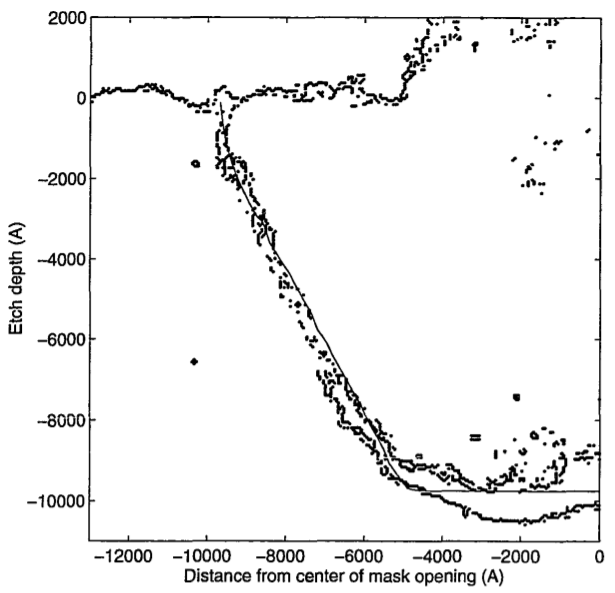
\includegraphics[scale = 0.8]{Figure 5.24}
	\bf\caption{  Comparison of extracted edge profile with results from string simulation (solid line).}
	\label{fig:5.24}
\end{figure}

\setstretch{1.5}

Completion of the response surface model will allow the implementation of the sidewallcontrol strategy presented in Section 5.1. First, the string model will be used to determine
the etch rate trajectories that must be followed to achieve a desired sidewall profile. The
response surface can then be used to translate these etch rate trajectories into the corresponding trajectories th at must be followed by the plasma characteristics. Finally, the
real-time controller can be used to force the plasma characteristics to follow these trajectories.

The implementation of this control strategy will provide a mechanism for translating
desired sidewall profiles into specific etch recipes. Once it is shown that this is possible, the work can be extended to more complicated etch situations. This may include using a more
industrially relevant masking layer, such as photoresist, and working with an etch process
which takes advantage of sidewall passivation.